\documentclass[a4paper,oneside,14pt]{extreport}

\usepackage[T2A]{fontenc}
\usepackage[utf8]{inputenc}
\usepackage[english,russian]{babel}

%\usepackage[left=30mm, right=20mm, top=20mm, bottom=20mm]{geometry}
\usepackage[left=20mm, right=10mm, top=5mm, bottom=20mm]{geometry}

\usepackage{microtype}
\sloppy

\usepackage{setspace}
\onehalfspacing

\usepackage{indentfirst}
\setlength{\parindent}{12.5mm}

\usepackage{titlesec}
\titleformat{\chapter}{\LARGE\bfseries}{\thechapter}{14pt}{\LARGE\bfseries}
\titlespacing*{\chapter}{\parindent}{0mm}{5mm}
\titleformat{\section}{\Large\bfseries}{\thesection}{14pt}{\Large\bfseries}

\addto{\captionsrussian}{\renewcommand*{\contentsname}{Содержание}}
\usepackage{natbib}
\renewcommand{\bibsection}{\chapter*{Список использованных источников}}

\usepackage{caption}

\usepackage{wrapfig}
\usepackage{float}

\usepackage{graphicx}
\newcommand{\imgwc}[4]
{
	\begin{figure}[#1]
		\center{\includegraphics[width=#2]{inc/img/#3}}
		\caption{#4}
		\label{img:#3}
	\end{figure}
}
\newcommand{\imghc}[4]
{
	\begin{figure}[#1]
		\center{\includegraphics[height=#2]{inc/img/#3}}
		\caption{#4}
		\label{img:#3}
	\end{figure}
}
\newcommand{\imgsc}[4]
{
	\begin{figure}[#1]
		\center{\includegraphics[scale=#2]{inc/img/#3}}
		\caption{#4}
		\label{img:#3}
	\end{figure}
}

\usepackage{pgfplots}
\pgfplotsset{compat=newest}

\usepackage{listings}
\usepackage{listingsutf8}
\lstset{
	basicstyle=\footnotesize\ttfamily,
	keywordstyle=\color{blue},
	stringstyle=\color{red},
	commentstyle=\color{gray},
	numbers=left,
	numberstyle=\tiny,
	numbersep=5pt,
	frame=false,
	breaklines=true,
	breakatwhitespace=true,
	inputencoding=utf8/koi8-r
}

\lstdefinestyle{c}{
	language=C++,
	backgroundcolor=\color{white},
	basicstyle=\footnotesize\ttfamily,
	keywordstyle=\color{blue},
	stringstyle=\color{red},
	commentstyle=\color{gray},
	directivestyle=\color{orange},
	numbers=left,
	numberstyle=\tiny,
	stepnumber=1,
	numbersep=5pt,
	frame=single,
	tabsize=4,
	captionpos=t,
	breaklines=true,
	breakatwhitespace=true,
	escapeinside={\#*}{*)},
	morecomment=[l][\color{magenta}]{\#},
	columns=fullflexible
}

\newcommand{\code}[1]{\texttt{#1}}

\usepackage{amsmath}
\usepackage{amssymb}

\usepackage[unicode]{hyperref}
\hypersetup{hidelinks}

\makeatletter
\newcommand{\vhrulefill}[1]
{
	\leavevmode\leaders\hrule\@height#1\hfill \kern\z@
}
\makeatother

\begin{document}

\begin{titlepage}
	\centering
	
	\vspace{-2.2mm}
	\vhrulefill{0.9mm}\\
	\vspace{-7mm}
	\vhrulefill{0.2mm}\\
	\vspace{2mm}
	
	\vspace{50mm}
	
	\vspace{30mm}
	
	\textbf{Отчет по лабораторной работе №7}\\
	По курсу: <<Фильтрация и прогнозирование данных>>\\
	Тема: <<Решение обратной задачи>>\\
	
	\vspace{60mm}
	
	\hspace{70mm} Студент:       \hfill Пронин~А.~С.\\
	\hspace{70mm} Группа:        \hfill МСМТ231\\
	\hspace{70mm} Преподаватель: \hfill Зотов~Л.~В.\\
	%	\hspace{70mm} Оценка:        \hfill \hrulefill\\
	
	\vfill
	
	Москва\\
	\the\year
\end{titlepage}

\setcounter{page}{2}

\chapter*{Лабораторная работа 2}
\section*{Задание 1 – Применить алгоритм скользящего среднего в частотной области}

Для начала применим алгоритм скользящего среднего в частотной области для сигнала из примера для проверки (рис. \ref{task1_not_my_signal}):

\begin{figure}[h]
	\center{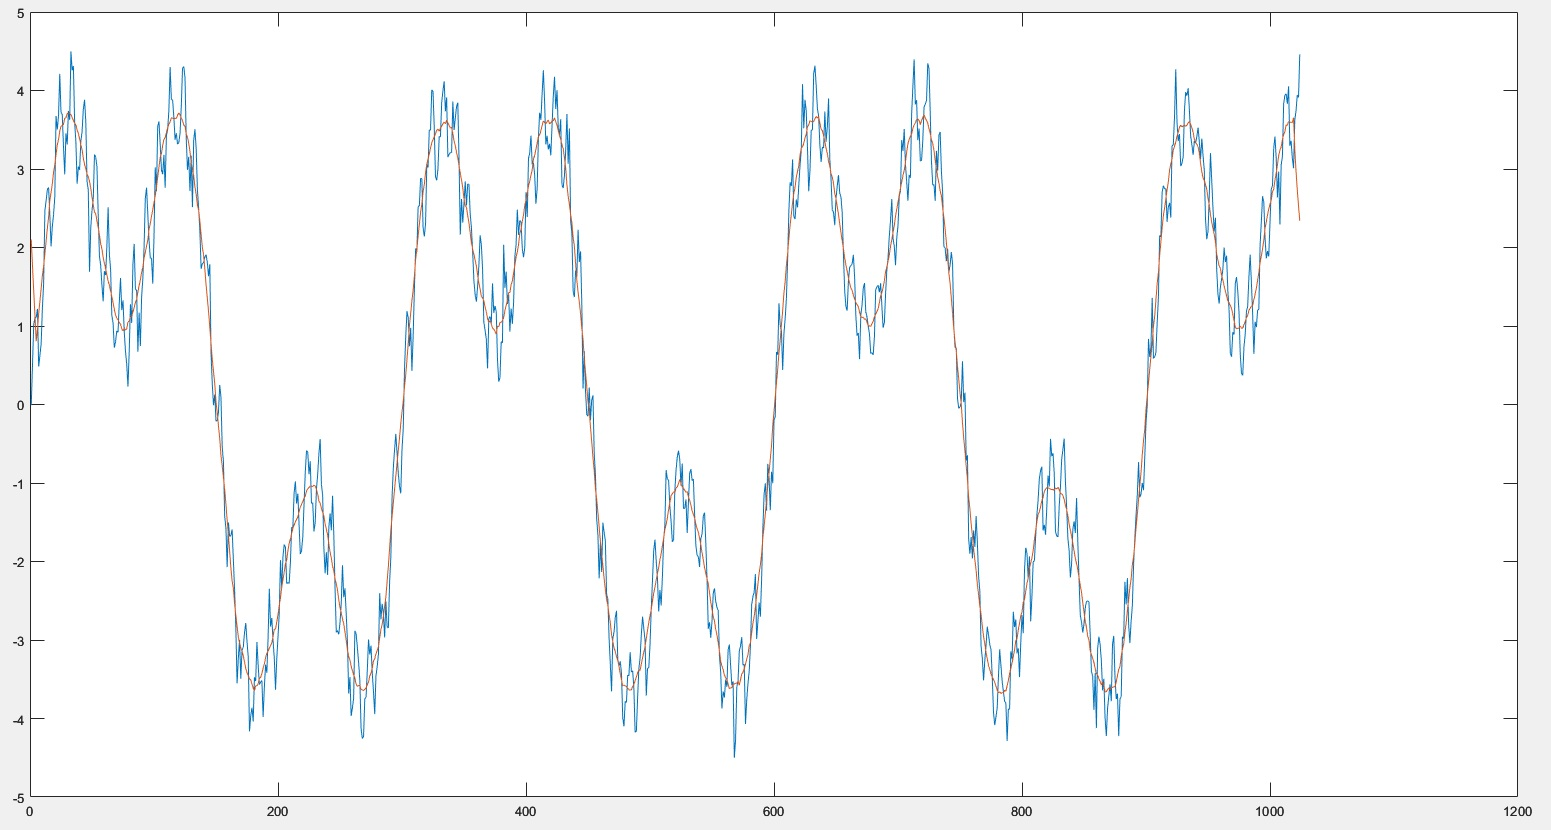
\includegraphics[width=1\linewidth]{inc/task1_not_my_signal}}
	\caption{Скользящее среднее в частотной области для сигнала из примера}
	\label{task1_not_my_signal}
\end{figure}

\newpage
Потом применим тот же метод для сигнала из первой лабораторной работы, с тем же размером окна 10 (рис. \ref{task1_my_signal}):

\begin{figure}[h]
	\center{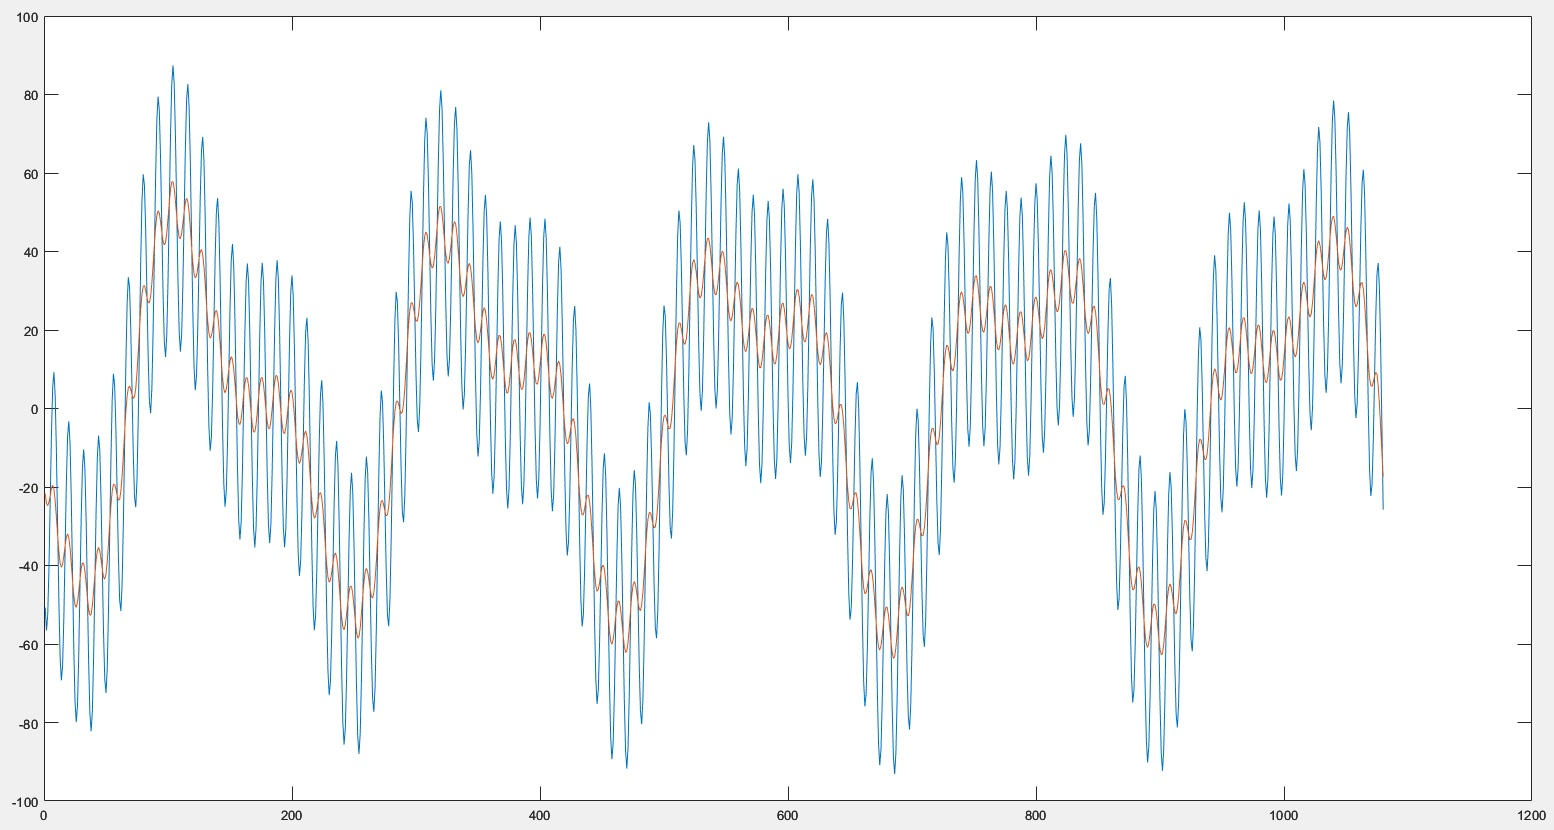
\includegraphics[width=1\linewidth]{inc/task1_my_signal}}
	\caption{Скользящее среднее в частотной области с размером окна 10}
	\label{task1_my_signal}
\end{figure}

Стоит обратить внимание что при использовании данного метода появляется краевой эффект из за того, что первые и последние $window\_size/2$ не имеют столько же соседей сколько другие точки и вычисленные в них значения сглаженного сигнала не корректны.

\newpage
\section*{Задание 2 – Изменить степень сглаживания}

Попробуем увеличить размер окна до 60 чтобы подавить высокочастотную гармонику рис. (рис. \ref{task2_my_signal}):

\begin{figure}[h]
	\center{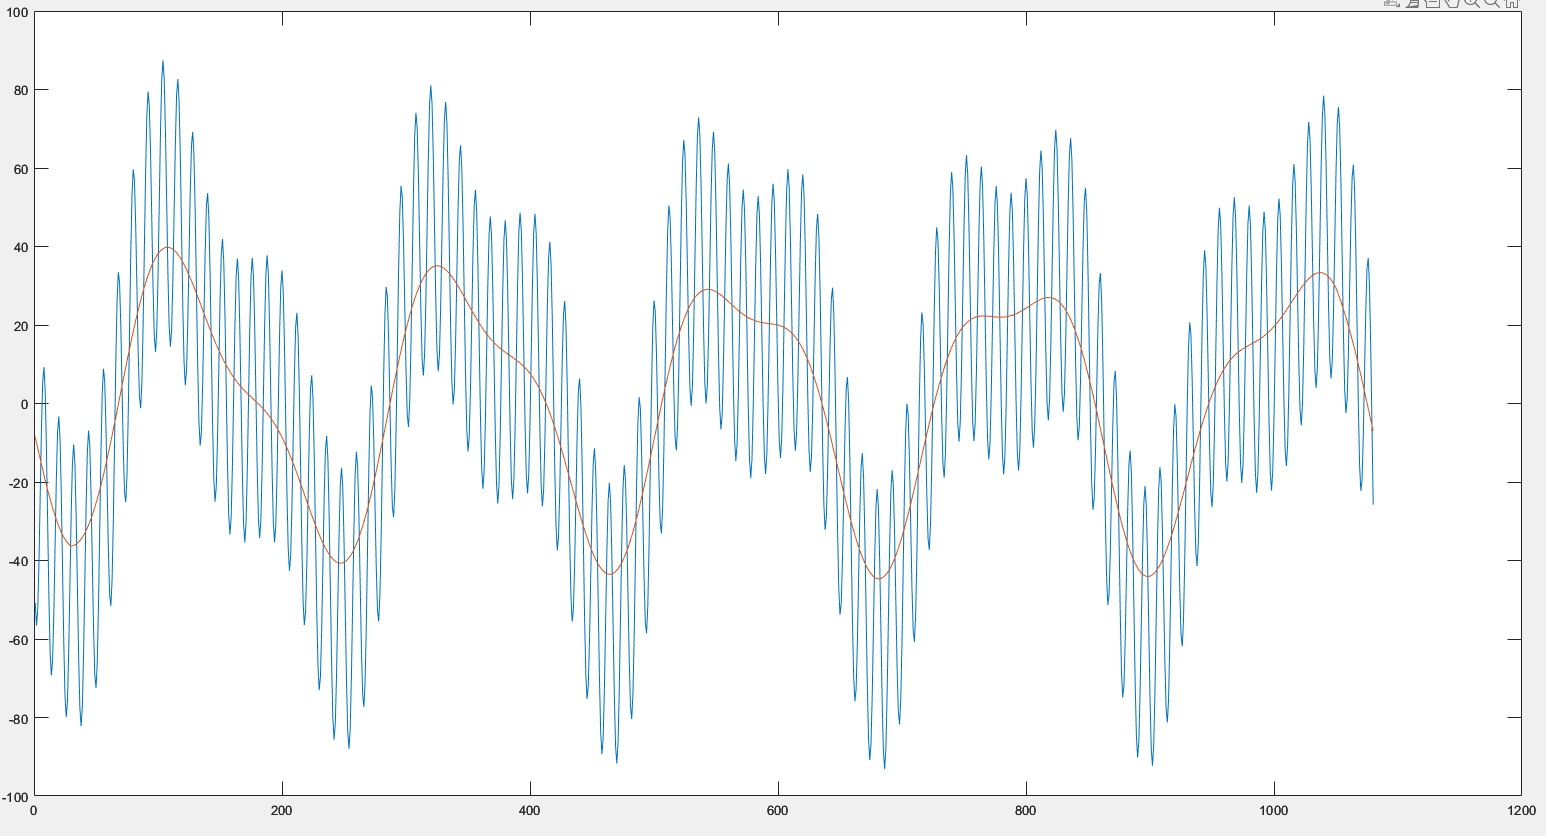
\includegraphics[width=1\linewidth]{inc/task2_my_signal}}
	\caption{Скользящее среднее в частотной области с размером окна 60}
	\label{task2_my_signal}
\end{figure}

\newpage
\section*{Задание 3 – Сравнить методы сглаживания во временной и частотной областях}

Теперь применим скользящее среднее во временной области, сначала для сигнала из примера с размером окна 20 для проверки (рис. \ref{task3_not_my_signal}):

\begin{figure}[h]
	\center{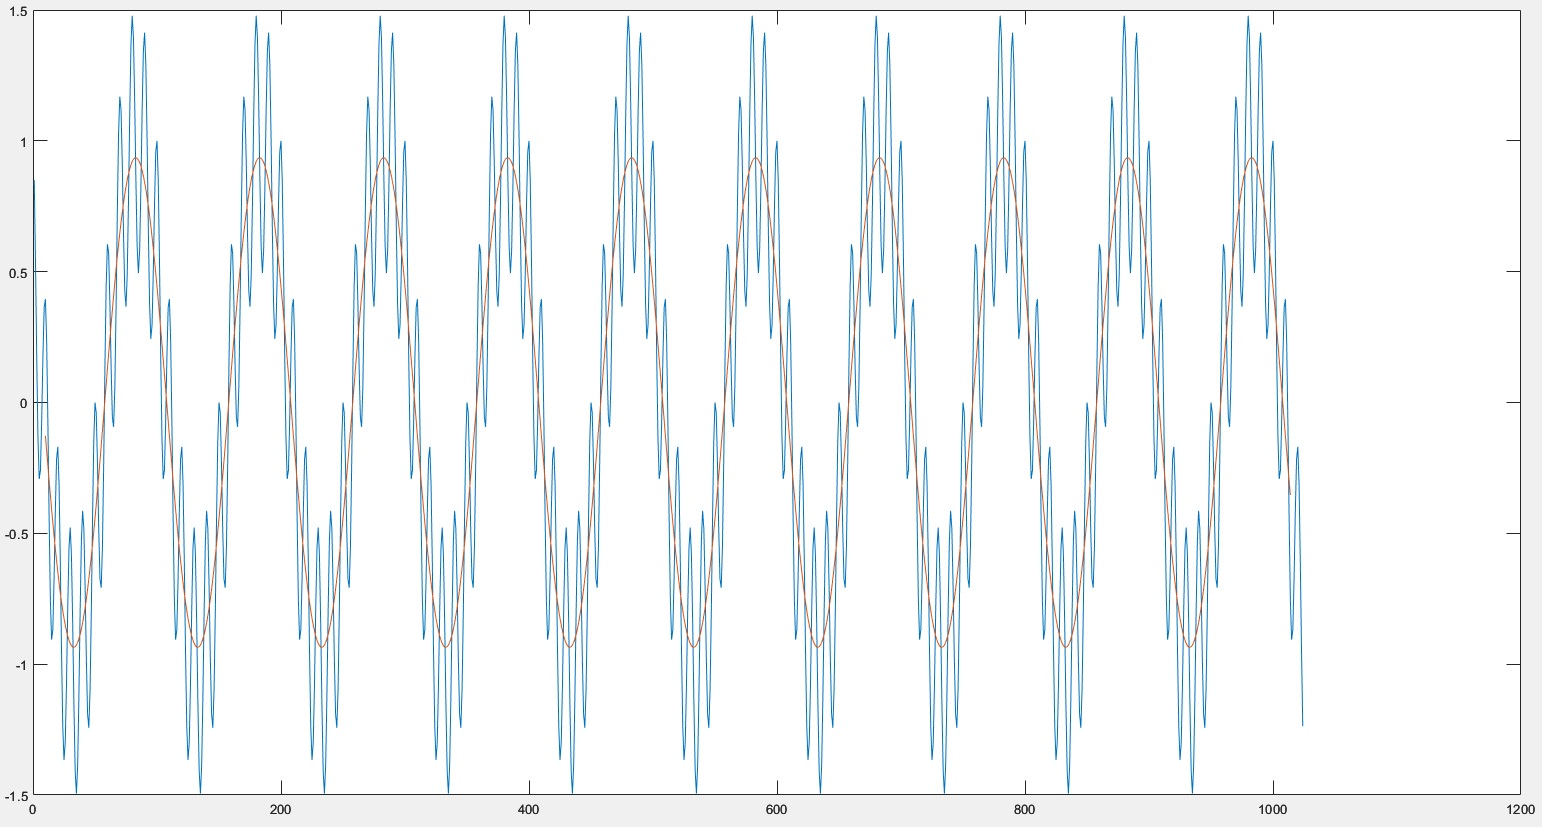
\includegraphics[width=1\linewidth]{inc/task3_not_my_signal}}
	\caption{Скользящее среднее во временной области для сигнала из примера}
	\label{task3_not_my_signal}
\end{figure}

\newpage
Затем применим тот же метод для нашего сигнала из первой лабораторной работы, с тем же размером окна 20 (рис. \ref{task3_my_signal}):

\begin{figure}[h]
	\center{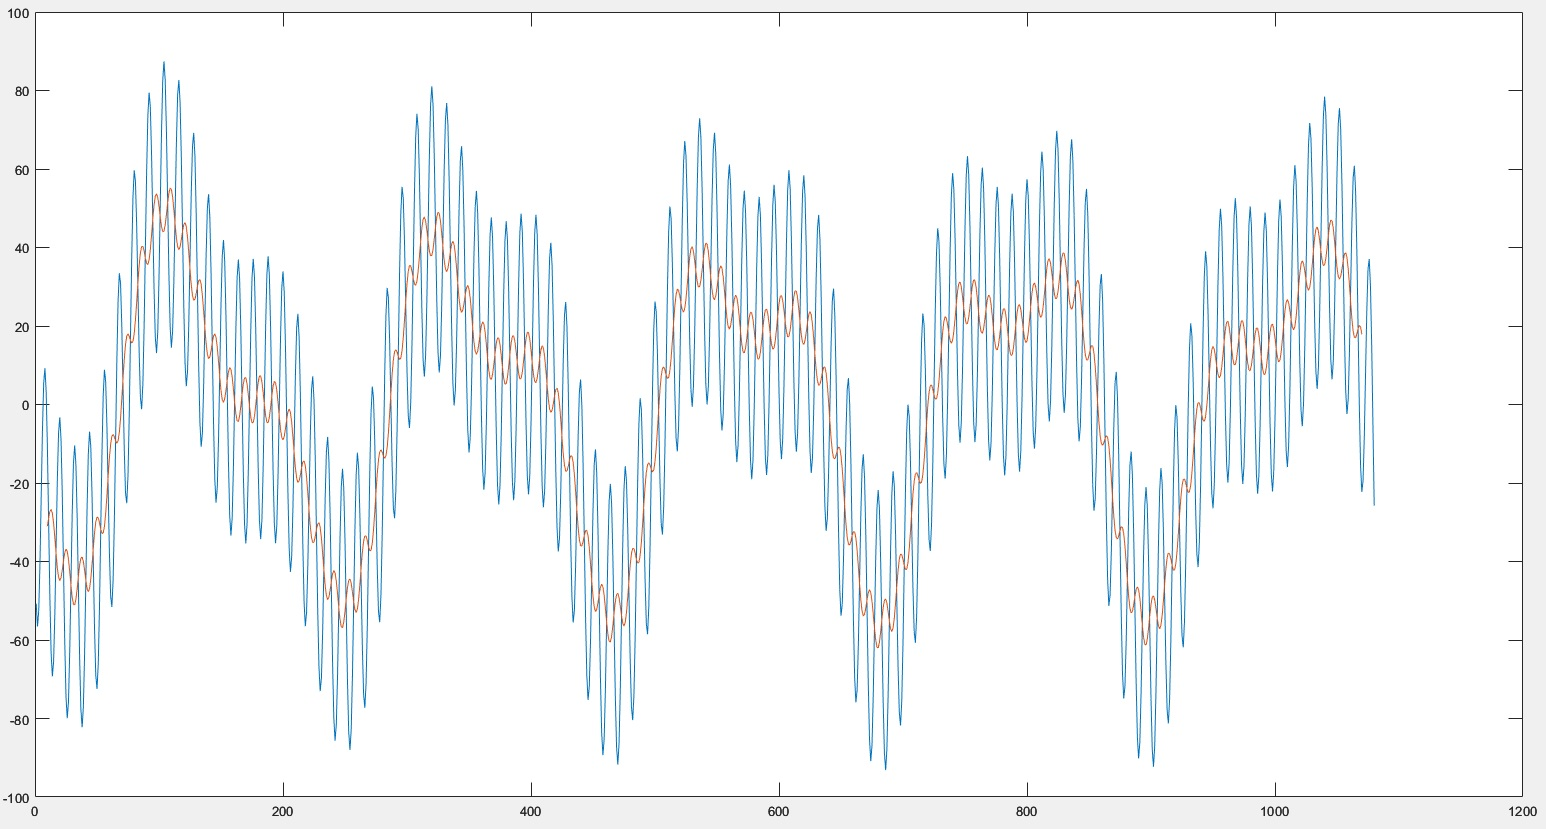
\includegraphics[width=1\linewidth]{inc/task3_my_signal}}
	\caption{Скользящее среднее во временной области с размером окна 20}
	\label{task3_my_signal}
\end{figure}

Здесь стоит отметить что в результате получается на $window\_size$ меньше элементов чем в исходном сигнале и их нужно смещать на $window\_size/2$ точек.

\newpage
Попробуем увеличить размер окна до 60 и сравним методы сглаживания во временной и частотной областях (рис. \ref{task3_my_signal2}-\ref{task2_my_signal2}):

\begin{figure}[h]
	\center{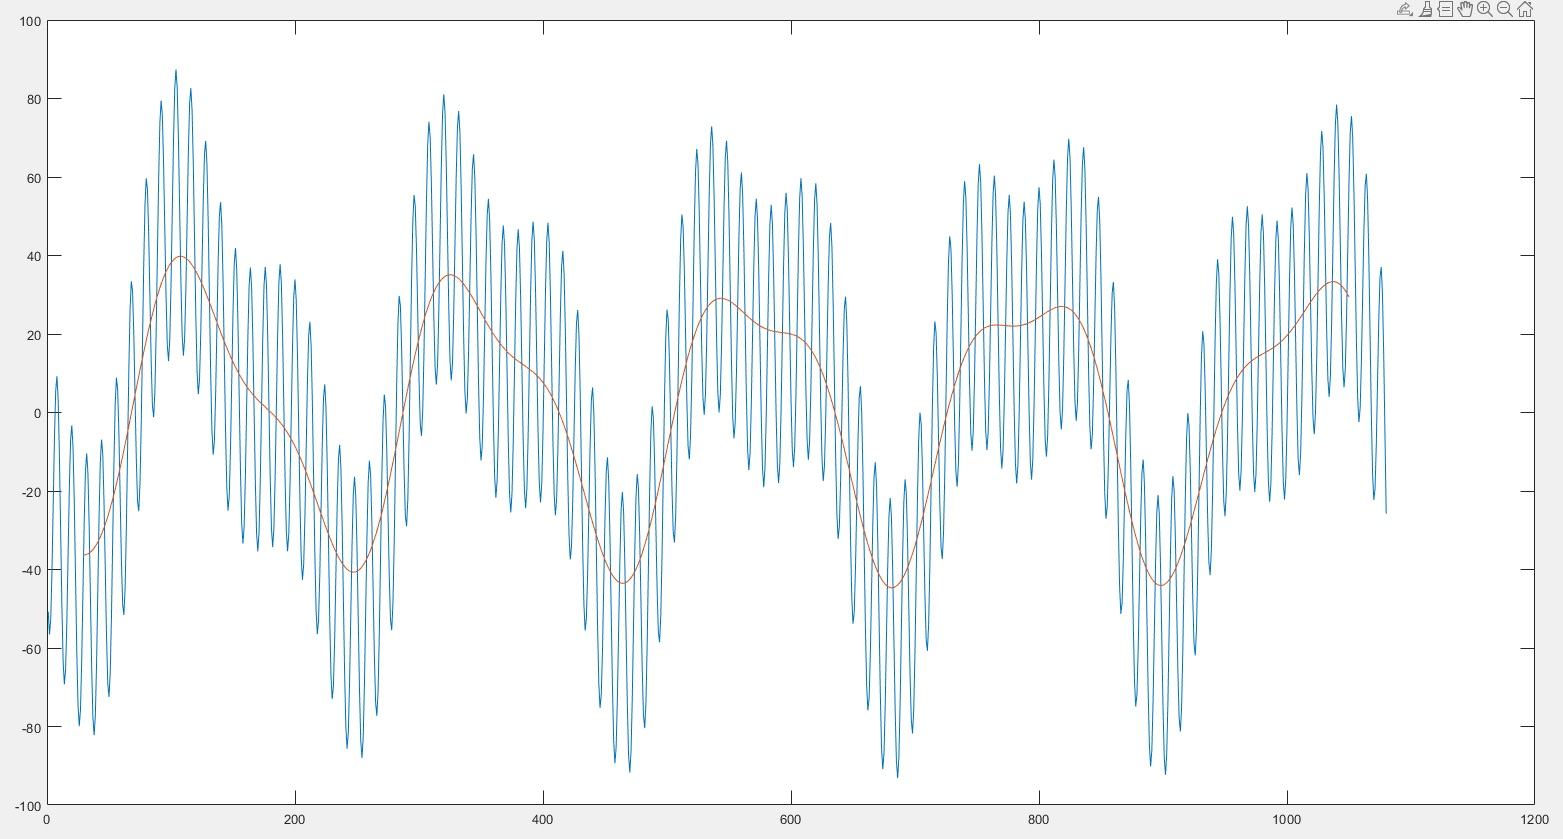
\includegraphics[width=0.95\linewidth]{inc/task3_my_signal2}}
	\caption{Скользящее среднее во временной области с размером окна 60}
	\label{task3_my_signal2}
\end{figure}

\begin{figure}[h]
	\center{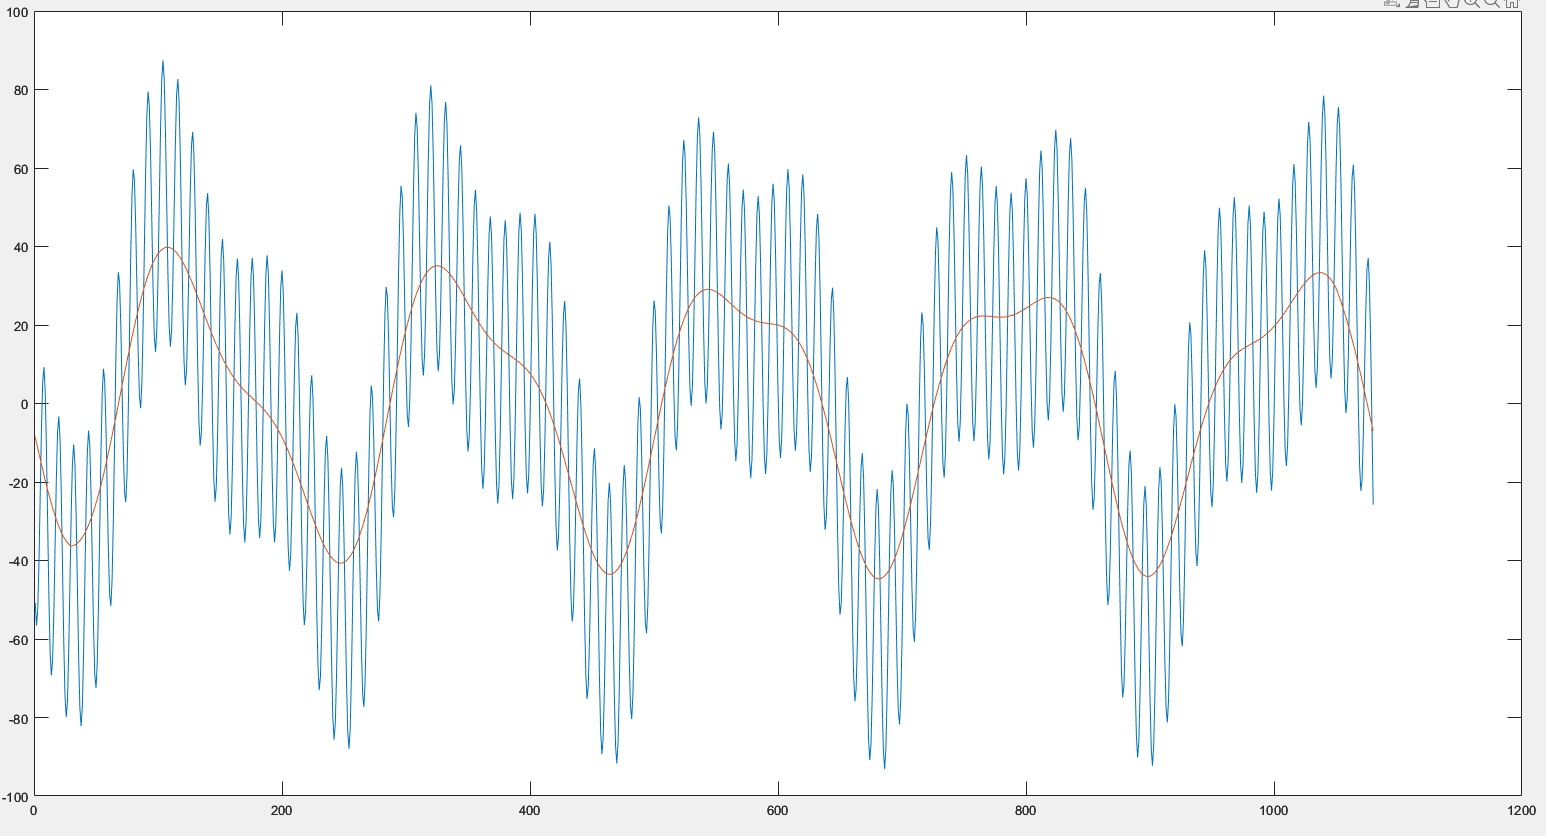
\includegraphics[width=0.9\linewidth]{inc/task2_my_signal}}
	\caption{Скользящее среднее в частотной области с размером окна 60}
	\label{task2_my_signal2}
\end{figure}

Как видно по графикам (рис. \ref{task3_my_signal2}-\ref{task2_my_signal2}) результат двух разных методов очень схож, но при использовании векторно-матричной свертки отсутствует краевой эффект, т.к. в нем не расчитываются значения для первых и последних $window\_size/2$ точек.

\end{document}